\documentclass{beamer}

\usepackage[utf8]{inputenc}
\usepackage{fancybox,fancyvrb}
\usepackage{environ}
\usepackage{tikz}

\beamertemplatenavigationsymbolsempty
\setbeamertemplate{footline}[frame number]
\usetheme{Pittsburgh}

\newcommand\enumnum[1]{{\renewcommand{\insertenumlabel}{#1}%
      \usebeamertemplate{enumerate item} \,}}

\newcommand{\grad}{\nabla}
\newcommand{\ih}{\boldsymbol{\hat{\textbf{\i}}}}
\newcommand{\jh}{\boldsymbol{\hat{\textbf{\j}}}}
\newcommand{\vF}{\boldsymbol{\vec{\textbf{F}}}}
\newcommand{\Matlab}{\textsc{Matlab}}


\title{4.3 Homogeneous linear equations \\ with constant coefficients}

\subtitle{a lesson for MATH F302 Differential Equations}

\author{Ed Bueler, Dept.~of Mathematics and Statistics, UAF}

\date{\tiny \today}


\begin{document}
\setbeamertemplate{itemize item}{$\bullet$}
\setbeamertemplate{itemize subitem}{$\circ$}


\begin{frame}
\titlepage

\centerline{\tiny for textbook: \, D. Zill, \emph{A First Course in Differential Equations with Modeling Applications}, 11th ed.}
%\color{green!40!blue}
\end{frame}


\begin{frame}{linear, homogeneous, constant-coefficient}

\begin{itemize}
\item recall from previous slides: \underline{linear} DEs which are \underline{homogeneous} and \underline{constant-coefficient} always have exponential solutions
    \begin{itemize}
    \item you can always find at least one solution $y=e^{mx}$
    \item the \underline{underlined} words are all important!
    \end{itemize}
\item \emph{example 1}: solve the ODE IVP
    $$y'' -2 y' - 4 y = 0, \quad y(-1)=4, \, y'(-1)=0$$

\vspace{30mm}
\end{itemize}
\end{frame}


\begin{frame}{example 1, finished}

\vspace{35mm}

\hfill 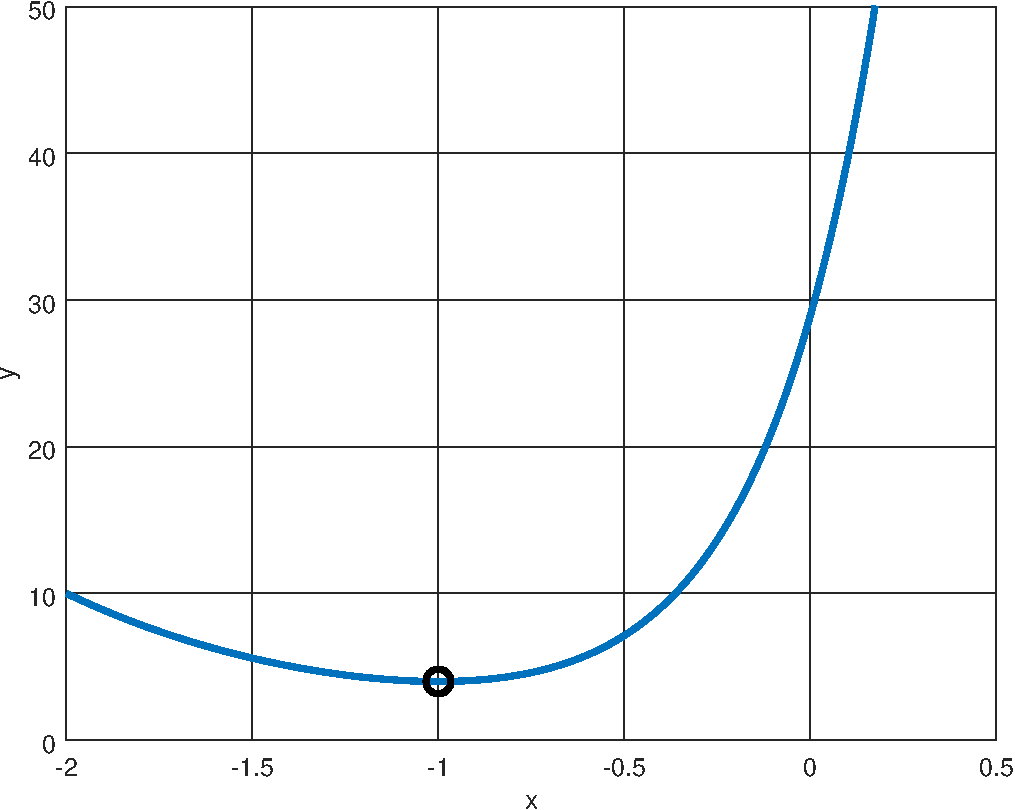
\includegraphics[width=0.5\textwidth]{figs/expodeivp2nd}
\end{frame}



\begin{frame}[fragile]
\frametitle{example 1: how I did it}

\begin{itemize}
\item I am committed to helping you use a computer for math, so here is how I made the last figure using \Matlab:

\bigskip
\begin{Verbatim}[fontsize=\small]
w = 1-sqrt(5);  z = 1+sqrt(5);
A = [exp(-w), exp(-z); w*exp(-w), z*exp(-z)];
b = [4; 0];
c = A \ b           % get: c(1)=0.8409, c(2)=28.119

x = -2:.01:1;
y = c(1) * exp(w*x) + c(2) * exp(z*x); 
plot(x,y),  grid on,  xlabel x,  ylabel y
axis([-2 0.5 0 50])
hold on,  plot(-1,4,'ko','markersize',12),  hold off
\end{Verbatim}
\end{itemize}
\end{frame}




\begin{frame}{expectations}

\begin{itemize}
\item just watching this video is \emph{not} enough!
     \begin{itemize}
     \item see ``found online'' videos at

     \centerline{\href{https://bueler.github.io/math302/week6.html}{\tt \color{cyan} bueler.github.io/math302/week6.html}}
     \item \emph{read} section 4.3 in the textbook
         \begin{itemize}
         \item for \S4.3 you at least need to know these terms:

\medskip
             \begin{tabular}{ll}
             \emph{homogeneous} \\
             \emph{linearly (in)dependent} \\
             \emph{Wronskian} \\
             \emph{fundamental set of solutions} \\
             \emph{linear combination} \\
             \emph{general solution}
             \end{tabular}

\bigskip
         \item why the repeated-roots case generates additional linearly-independent solutions by extra factors of ``$x$'' is explained in \S4.2
         \end{itemize}
     \item \emph{do} the WebAssign exercises for section 4.3
     \end{itemize}
\end{itemize}
\end{frame}

\end{document}

